%
% This is the LaTeX template file for lecture notes for CS294-8,
% Computational Biology for Computer Scientists.  When preparing 
% LaTeX notes for this class, please use this template.
%
% To familiarize yourself with this template, the body contains
% some examples of its use.  Look them over.  Then you can
% run LaTeX on this file.  After you have LaTeXed this file then
% you can look over the result either by printing it out with
% dvips or using xdvi.
%
% This template is based on the template for Prof. Sinclair's CS 270.

\documentclass{article}
\usepackage{graphics}
\usepackage{multicol}
\usepackage{tikz}
\usepackage{clrscode3e}
\usepackage{enumitem}
\usepackage{amsmath}
\usepackage{amsthm}
\usepackage{amssymb}

\setlength{\oddsidemargin}{0 in}
\setlength{\evensidemargin}{0 in}
\setlength{\topmargin}{-0.6 in}
\setlength{\textwidth}{6.5 in}
\setlength{\textheight}{8.5 in}
\setlength{\headsep}{0.75 in}
\setlength{\parindent}{0 in}
\setlength{\parskip}{0.1 in}

%
% The following commands set up the lecnum (lecture number)
% counter and make various numbering schemes work relative
% to the lecture number.
%
\newcounter{lecnum}
\renewcommand{\thepage}{\thelecnum-\arabic{page}}
\renewcommand{\thesection}{\thelecnum.\arabic{section}}
\renewcommand{\theequation}{\thelecnum.\arabic{equation}}
\renewcommand{\thefigure}{\thelecnum.\arabic{figure}}
\renewcommand{\thetable}{\thelecnum.\arabic{table}}

%
% The following macro is used to generate the header.
%
\newcommand{\lecture}[4]{
   \pagestyle{myheadings}
   \thispagestyle{plain}
   \newpage
   \setcounter{lecnum}{#1}
   \setcounter{page}{1}
   \noindent
   \begin{center}
   \framebox{
      \vbox{\vspace{2mm}
    \hbox to 6.28in { {\bf CSC2420 - Algorithm Design, Analysis and Theory
                        \hfill Fall 2022} }
       \vspace{4mm}
       \hbox to 6.28in { {\Large \hfill Lecture #1: #2  \hfill} }
       \vspace{2mm}
       \hbox to 6.28in { {\it Lecturer: #3 \hfill Scribe: #4} }
      \vspace{2mm}}
   }
   \end{center}
   \markboth{Lecture #1: #2}{Lecture #1: #2}
   % {\bf Disclaimer}: {\it These notes have not been subjected to the
   % usual scrutiny reserved for formal publications.  They may be distributed
   % outside this class only with the permission of the Instructor.}
   \vspace*{4mm}
}

%
% Convention for citations is authors' initials followed by the year.
% For example, to cite a paper by Leighton and Maggs you would type
% \cite{LM89}, and to cite a paper by Strassen you would type \cite{S69}.
% (To avoid bibliography problems, for now we redefine the \cite command.)
% Also commands that create a suitable format for the reference list.
\renewcommand{\cite}[1]{[#1]}
\def\beginrefs{\begin{list}%
        {[\arabic{equation}]}{\usecounter{equation}
         \setlength{\leftmargin}{2.0truecm}\setlength{\labelsep}{0.4truecm}%
         \setlength{\labelwidth}{1.6truecm}}}
\def\endrefs{\end{list}}
\def\bibentry#1{\item[\hbox{[#1]}]}

%Use this command for a figure; it puts a figure in wherever you want it.
%usage: \fig{NUMBER}{SPACE-IN-INCHES}{CAPTION}
\newcommand{\fig}[3]{
			\vspace{#2}
			\begin{center}
			Figure \thelecnum.#1:~#3
			\end{center}
	}
% Use these for theorems, lemmas, proofs, etc.
\newtheorem{theorem}{Theorem}[lecnum]
\newtheorem{lemma}[theorem]{Lemma}
\newtheorem{proposition}[theorem]{Proposition}
\newtheorem{claim}[theorem]{Claim}
\newtheorem{corollary}[theorem]{Corollary}
\newtheorem{definition}[theorem]{Definition}
\newtheorem{problem}[theorem]{Problem}
\newtheorem{conjecture}[theorem]{Conjecture}
\renewenvironment{proof}{{\bf Proof:}}{\hfill\rule{2mm}{2mm}}

\newcommand{\Exp}{\mathbb{E}}
\newcommand{\Var}{\mathrm{Var}}


\begin{document}
%FILL IN THE RIGHT INFO.
%\lecture{**LECTURE-NUMBER**}{**DATE**}{**LECTURER**}{**SCRIBE**}
\lecture{9}{Vector Program and Random Walk}{Allan Borodin}{Kevin Gao}

\section{SDP and Vector Program for Max-2-SAT}

We consider the formulation of max-2-SAT as a \textbf{semidefinite programming} (SDP) problem.

We introduce the variables $y_i$ where
$$
\begin{array}{ll}
    y_i = \pm 1 & \text{for $i = 0,\ldots,m$ } \\
    y_i = y_0 & \text{iff $x_i$ is true}
\end{array}
$$
To define the objective function, we want each clause $C$ to have a value 1 if the clause is satisfied and 0 otherwise:
$$
\begin{aligned}
    v(x_i) &= \frac{1 + y_i y_0}{2} \\
    v(\neg x_i) &= \frac{1 - y_i y_0}{2} \\
    v(x_i \lor x_j) &= 1 - v(\neg x_i) v(\neg x_j) = \frac{1 + y_0y_i}{4} + \frac{1 + y_0y_j}{4} + \frac{1 - y_iy_j}{4} \\
    v(\neg x_i \lor x_j) &= \frac{3 - y_i y_0 + y_jy_0 + y_iy_j}{4} \\
    v(\neg x_i \lor \neg x_j) &= \frac{3 - y_iy_0 - y_jy_0 - y_iy_j}{4}
\end{aligned}
$$
We can then define the objective as
$$
\begin{array}{lll}
    \max & \sum_{k} w_k v(C_k) \\
    \text{s.t.} & y_i^2 = 1 & \forall i \in \{0,\ldots,m\}
\end{array}
$$
By collecting like terms, the objective can be expressed equivalently as
$$
\max \sum_{0 \leq i < j \leq n} a_{ij} (1 + y_iy_j) + \sum_{0 \leq i < j \leq n} b_{ij} (1 - y_iy_j)
$$
for some appropriate $a_{ij}$ and $b_{ij}$.

We now relax the quadratic program to a vector program where each $y_i$ is now a unit length vector $\mathbf{v}_i$ in $\mathbb{R}^{n+1}$ and scalar multiplication is replaced by vector dot product. This vector program can be approximated in polynomial time.
$$
\max \sum_{0 \leq i,j \leq n} a_{ij} (1 + \mathbf{v}_i \cdot \mathbf{v}_j) + b_{ij} (1 - \mathbf{v}_i \cdot \mathbf{v}_j) \qquad \mathbf{v}_i \in \mathbb{R}^{n+1},\, \lVert \mathbf{v}_i \rVert = 1
$$

The randomized rounding proceeds by choosing a random hyperplane in $\mathbb{R}^{n+1}$ and then setting $y_i = 1$ if and only if $\mathbf{v}_i^*$ is on the same side of the hyperplane as $\mathbf{v}_0^*$. That is, let $\mathbf{r}$ is a uniform random vector in $\mathbb{R}^{n+1}$, and then set $y_1 = 1$ if and only if $\mathbf{r} \cdot \mathbf{v}_i^* \geq 0$.

\begin{theorem}
    The vector program relaxation is a 0.8785-approximation for Max-2-SAT.
\end{theorem}

\begin{proof}
    The expected weight produced by the randomly rounded vector program is
    $$
    \Exp[W] = \sum_{0\leq i,j \leq n} a_{ij} (1 + \Exp[y_i \cdot y_j]) + b_{ij} (1 - \Exp[y_i \cdot y_j])
    $$
    where
    $$
    \Exp[y_i \cdot y_j] = \Pr[y_i = y_j] \cdot 1 + \Pr[y_i \neq y_j] \cdot (-1)
    $$
    We claim that
    $$
    \Pr[y_i \neq y_j] = \frac{\theta_{ij}}{\pi}
    $$
    Let $\mathbf{r}$ be a random vector and $\mathbf{s}$ be the projection of $\mathbf{r}$ onto the plane containing $\mathbf{v}_i$ and $\mathbf{v}_j$. Then,
    $$
    \begin{aligned}
        \mathbf{v}_i \cdot \mathbf{r} &= \mathbf{v}_i \cdot (\mathbf{s} + \mathbf{r} - \mathbf{s}) \\
        &= \mathbf{v}_i \cdot \mathbf{s} + \mathbf{v}_i \cdot (\mathbf{r} - \mathbf{s}) \\
        &= \mathbf{v}_i \cdot \mathbf{s}
    \end{aligned}
    $$
    Note that the second term vanishes because $\mathbf{r}-\mathbf{s}$ is orthogonal to $\mathbf{v}_i$. By the same argument, $\mathbf{v}_j \cdot \mathbf{r} = \mathbf{v}_i \cdot \mathbf{s}$. Now, $y_i$ and $y_j$ are set to different values iff $\mathbf{v}_i$ and $\mathbf{v}_j$ are separated by the hyperplane defined by $\mathbf{r}$. Hence, it suffices to consider the probability $\Pr[\text{$\mathbf{v}_i$ and $\mathbf{v}_j$ are separated}]$.
    
    Without loss of generality, suppose that $\mathbf{v}_i$ has angular coordinate $0$ and $\mathbf{v}_j$ has angular coordinate $\theta_{ij}$. Further, let $\phi$ denote the angular coordinate of $\mathbf{s}$.

    \begin{figure}[htbp]
        \centering
        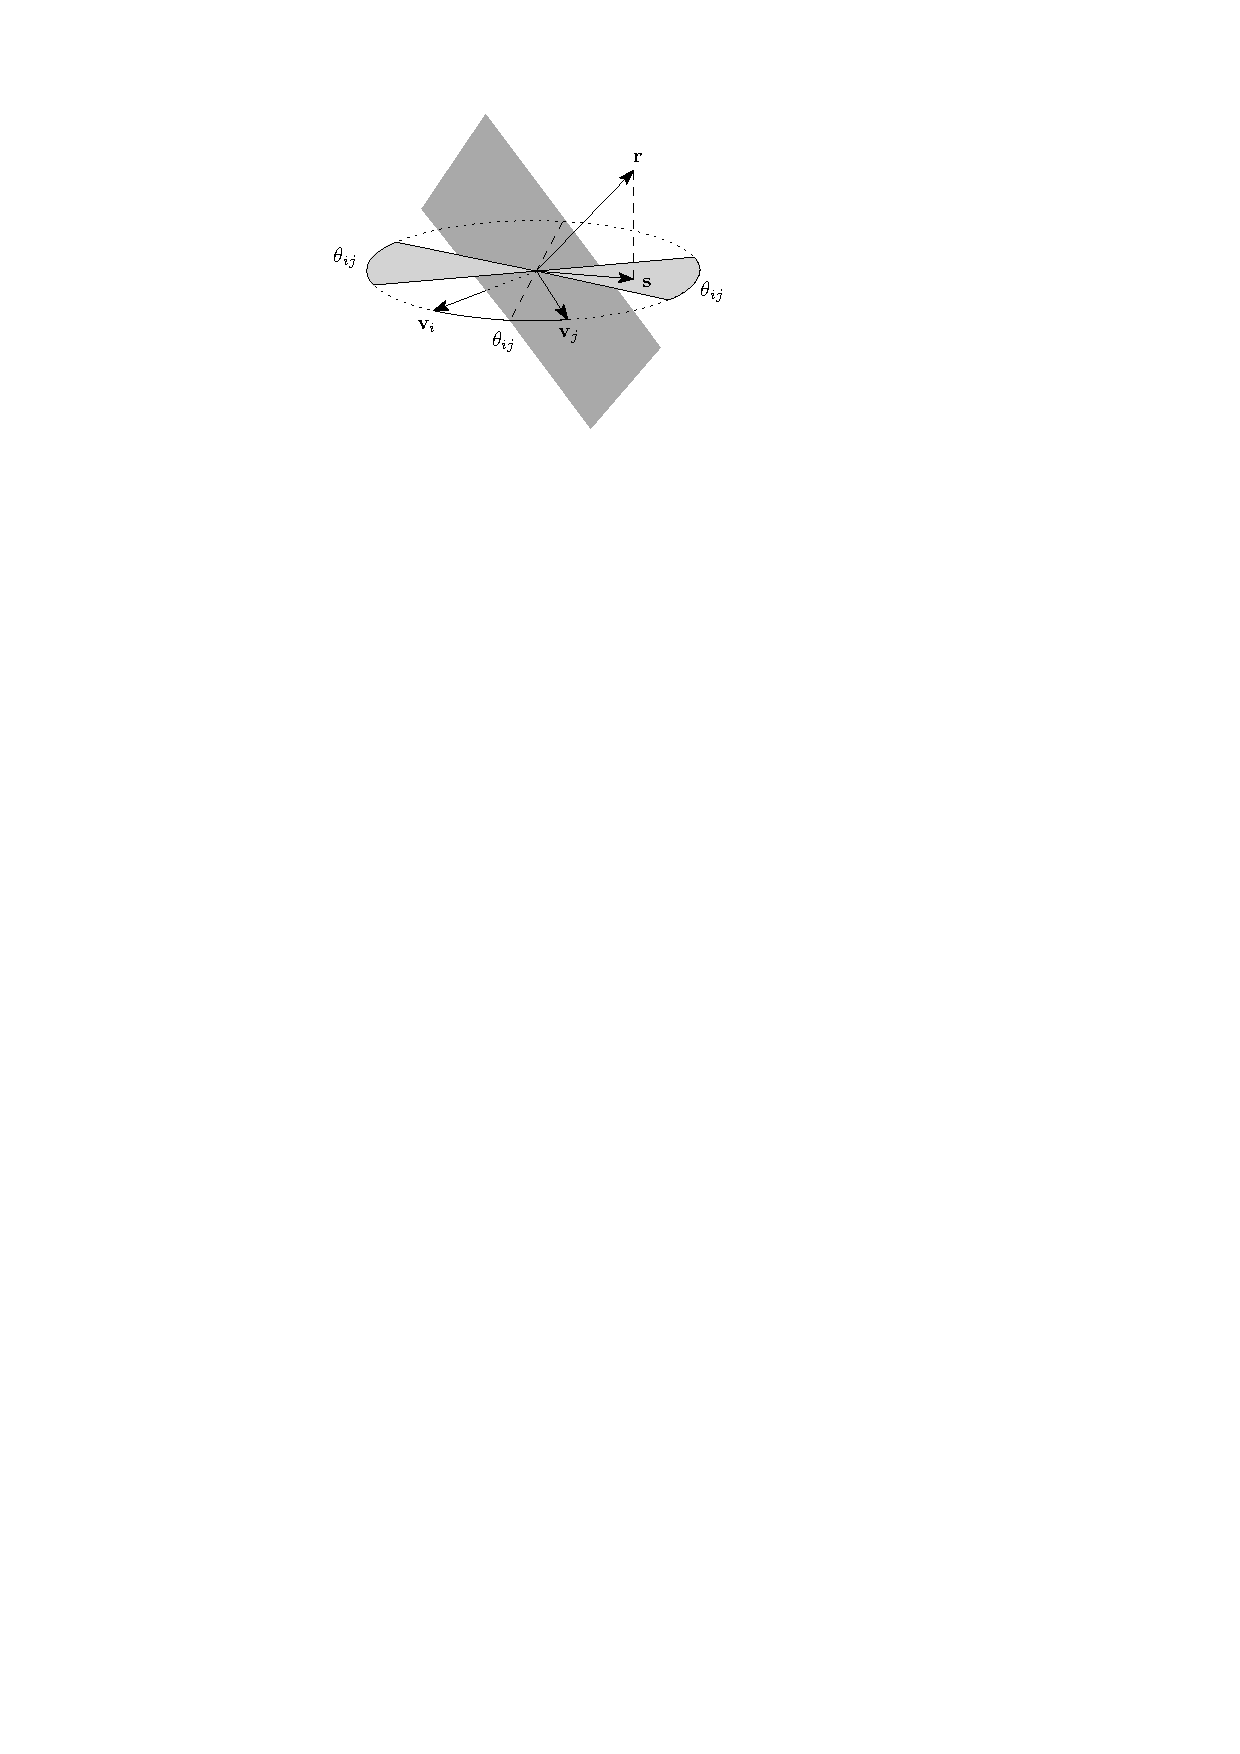
\includegraphics[width=0.4\linewidth]{hyperplane-rounding.pdf}
        \caption{A random hyperplane defined by $\mathbf{r}$ separating $\mathbf{v}_j$ and $\mathbf{v}_i$.}
    \end{figure}

    $\mathbf{v}_i$ and $\mathbf{v}_j$ are separated by the hyperplane whenever $\mathbf{s}$ is within the lightly shaded region. There are two such regions, each with angular diameter $\theta_{ij}$. Since $\mathbf{r}$ is uniformly chosen from $\mathbb{R}^{n+1}$, its projection $\mathbf{s}$ is uniformly distributed over $[0,2\pi)$. There are two slices of diameter $\theta_{ij}$ that $\mathbf{s}$ can be in so that the hyperplane separate $\mathbf{v}_i$ and $\mathbf{v}_j$. Hence,
    $$
    \Pr[\text{$\mathbf{v}_i$ and $\mathbf{v}_j$ are separated}] = \frac{2 \cdot \theta_{ij}}{2\pi} = \frac{\theta_{ij}}{\pi}.
    $$
    It follows that $\Pr[y_i = y_j] = \frac{\theta_{ij}}{\pi} = 1 - \frac{\theta_{ij}}{\pi}$. 
    
    We define
    $$
    \alpha = \frac{2}{\pi} \min_{0 \leq \theta \leq \pi} \frac{\theta}{1 - \cos\theta} \approx 0.87856
    $$
    Observe that from calculus, we have for $0 \leq \theta \leq \pi$,
    $$
    \frac{\theta}{\pi} \geq \alpha \left( \frac{1 - \cos\theta}{2} \right) 
    $$
    and similarly, for $0 \leq \theta \leq \pi$, $1 - \frac{\theta}{\pi} \geq \alpha \left( \frac{1 + \cos\theta}{2} \right)$. Then,
    $$
    \begin{aligned}
        \Exp[W] &= \sum_{0\leq i,j \leq n} a_{ij} (1 + \Exp[y_i \cdot y_j]) + b_{ij} (1 - \Exp[y_i \cdot y_j]) \\
        &= \sum_{0 \leq i,j \leq n} a_{ij} \left( 2 - \frac{2\theta_{ij}}{\pi} \right) + b_{ij} \cdot \frac{2\theta_{ij}}{\pi} \\
        &= \sum_{0 \leq i,j \leq n} 2 a_{ij} \left( 1 - \frac{\theta_{ij}}{\pi} \right) + 2 b_{ij} \cdot \frac{\theta_{ij}}{\pi} \\
        &\geq \sum_{0 \leq i,j \leq n} 2 a_{ij} \left( \frac{1 + \cos\theta_{ij}}{2} \right) + 2 b_{ij} \cdot \left( \frac{1 - \cos\theta_{ij}}{2} \right)
    \end{aligned}
    $$
    Finally, since $\mathbf{v}_i \cdot \mathbf{v}_j = \lVert \mathbf{v}_i \rVert \cdot \lVert \mathbf{v}_j \rVert \cdot \cos\theta_{ij}$ and $\lVert \mathbf{v}_i \rVert = \lVert \mathbf{v}_j \rVert = 1$,
    $$
    \begin{aligned}
        \Exp[W] &\geq  \sum_{0 \leq i,j \leq n} 2 a_{ij} \left( \frac{1 + \cos\theta_{ij}}{2} \right) + 2 b_{ij} \cdot \left( \frac{1 - \cos\theta_{ij}}{2} \right) \\
        &= \sum_{0 \leq i,j \leq n} 2 a_{ij} \left( \frac{1 + \mathbf{v}_i \cdot \mathbf{v}_j}{2} \right) + 2 b_{ij} \cdot \left( \frac{1 - \mathbf{v}_i \cdot \mathbf{v}_j}{2} \right) \\
        &= \sum_{0 \leq i,j \leq n} a_{ij} \left( {1 + \mathbf{v}_i \cdot \mathbf{v}_j} \right) + b_{ij} \cdot \left( {1 - \mathbf{v}_i \cdot \mathbf{v}_j} \right) \\
        &=  \alpha \cdot OPT_{\mathrm{VP}} \\
        &\geq \alpha \cdot OPT_{\mathrm{SDP}} \\
    \end{aligned}
    $$
\end{proof}

\section{SAT}

\subsection{Polynomial-time Algorithm for 2-SAT}

Consider a 2CNF formula $F$ in $n$ variables. We consider each clause $x \lor y$ as an implication $\neg x \implies y$ and $\neg y \implies x$. We then construct a directed graph on $2n$ nodes corresponding to the $2n$ literals and edges corresponding to the implications above. For example, $x \implies y$ induces an edge $(x,y)$. We claim that $F$ is satisfiable iff there does not exist a variable $x$ such that there is a directed path from $x$ to $\neg x$ and a path $\neg x$ to $x$.

Clearly, $k$-SAT (for CNF formula with $n$ variables, $m$ clauses, and at most $k$ literals/clauses) cna be trivially decided in time $\widetilde{O}(2^n m)$. $\widetilde{O}$ is the soft-O notation, in which we drops lower order terms (including multiplicative log factors).

\subsection{3-SAT}

Consider a 3-CNF formula with $n$ variables and $m$ clauses. While there are any clauses with 3 literals (say, $x,y,z$), branch on each of the 7 possible settings for $(x,y,z)$ that can make the clause true (8 possible truth assignments, excluding the one that falsifies the clause).

On any branch, the current truth value setting can satisfy some clauses which can then be eliminated. In other clauses involving some variable in the current truth assignment, one or two variables can be eliminated. We repeat this until there are no clauses remaining with 3 literals. If any branch satisfies all clauses or if we are left with only consistent unit clauses, the given formula is satisfiable. If we are left with two contradictory unit clauses, the given formula is unsatisfiable.

The depth of the tree is at most $n / 3$ since we are eliminating 3 distinct variables at each level. Hence, the time complexity is
$$
O(7^{n/3} \mathit{poly}(m)) = 2^{\log_2 7n / 3} \mathit{poly}(m) \approx 2^{2.81n / 3} \mathit{poly}(m)
$$
This branch-and-bound algorithm is a slight improvement on the naive algorithm which tries all $2^n$ possible truth assignments.

\section{Random Walk for 2-SAT}

The randomized algorithm for 2-SAT is based on arandom walk on the line graph with nodes $\{0,1,\ldots,n\}$. Being on node $i$ can be interpreted as havinga truth assignment $\tau$ that is Hamming distance $i$ from some fixed satisfying assignment $\tau^*$ if $F$ is satisfiable.

Start with an arbitrary truth assignment $\tau$ and if $F(\tau)$ is true then we are done; else find an arbitrary unsatisfied clause $C$ and randomly choose one of the two variables $x_i$ occurring in $C$ and then change $\tau$ to $\tau'$ by setting $\tau'(x_i) = 1 - \tau(x_i)$.

Note that when we randomly select one of the two literals in $C$ and flip it, we are getting closer to $\tau^*$ with probability at least $1/2$. The distance to node 0 in a random walk on the line where on each random step, the distance to node 0 is reduced by 1 with at least $1/2$ probability and otherwise increased by 1.

\begin{theorem}
    The expected time to hit node 0 is at most $2n^2$.
\end{theorem}

\subsection{Markov Chain}

A \textbf{finite Markov chain} $M$ is a discrete-time random proces defined over a set of \textbf{states} $S$ and a matrix $\mathbf{P} = \{P_{ij}\}$ of \textbf{transition probabilities}.

Denote by $X_t$ the state of the Markov chain at time $t$. It is a memoryless process since the future behavior of a Markov chain \textit{depends only on its current state}:
$$
\Pr[X_{t+1} = j \mid X_t = i] = P_{ij}
$$
and hence
$$
\Pr[X_{t+1} = j] = \sum_{i} \Pr[X_{t+1} = j \mid X_t = i] \Pr[X_t = i]
$$
Given an initial state $i$, denote by $r_{ij}^t$ the probability that the first time the process reaches state $j$ occurs at time $t$.
$$
r_{ij}^t = \Pr[X_t = j \land X_s \neq j,\, 1 \leq s \leq t-1 \mid X_0 = i]
$$
Let $f_{ij}$ be the probability that state $j$ is reachable from initial state $j$.
$$
f_{ij} = \sum_{t > 0} r_{ij}^t
$$
Let $h_{ij}$ denote the expected number of steps to reach state $j$ starting from state $i$ (\textbf{hitting time}).
$$
h_{ij} = \sum_{t > 0} t \cdot r_{ij}^t
$$
Finally, the \textbf{commute time} $c_{ij}$ is the expected number of steps to reach state $j$ sstarting from state $i$, and then return from $i$ to $j$. That is,
$$
c_{ij} = h_{ij} + h_{ji}.
$$

The underlying directed graph of a Markov chain is a graph where each vertex in the graph corresponds to a state of the Markov chain
and there is a directed edge from vertex $i$ to vertex $j$ iff $P_{ij} > 0$. A Markov chain is \textbf{irreducible} if its underlying graph \textit{consists of a single strongly connected component}. We have the following theorem.

\begin{theorem}[Fundamental Theorem of Markov Chains]
    For any finite, irreducible, and aperiodic Markov chain, there exists a unique stationary distribution $\pi$ and for all states $i$, $h_{ii} < \infty$ and $h_{ii} = 1 / \pi_{i}$. 
\end{theorem}

\subsection{Random Walk on Graphs}

We can now use our knowledge of Markov chains to analyze the expected time of the random walk algorithm for 2-SAT.

Let $G=(V,E)$ be a connected, non-bipartite, undirected graph with $|V| = n$ and $|E| = m$. A uniform random walk induces a Markov chain $M_G$ where
\begin{itemize}
    \item the states of $M_G$ are the vertices
    \item for $u,v \in V$, $P_{uv} = 1 / \deg(u)$ if $(u,v) \in E$ and $P_{uv} = 0$ if $(u,v) \not\in E$
\end{itemize}
And
$$
\left( \frac{\deg(v_1)}{2m}, \ldots, \frac{\deg(v_n)}{2m} \right) 
$$
is a stationary distribution of $M_G$.

Define $\mathbf{q}^t = [ q_1^t\, q_2^t\, \ldots\, q_{n}^t ]$ as the state probability vector, which is a row vector whose $i$-th component is the probability that the Markov chain is in state $i$ at time $t$. A distribution $\pi$ is a stationary distribution for a Markov chain with transition matrix $\mathbf{P}$ if $\pi = \pi \mathbf{P}$.

Let $C_u(G)$ be the expected time to visit every vertex, starting from $u$. Also, $C(G) = \max_u C_u(G)$ to be the cover time for $G$.
\begin{theorem}[Aleliunas et al, 1979]
    Let $G$ be a connected undirected graph. Then, for each edge $(u,v)$, $C_{u,v} \leq 2m$. And $C(G) \leq 2m(n-1)$.
\end{theorem}
It follows from this theorem that the simple random walk algorithm for 2-SAT has expected time at most $2n^2$.

\subsection{Schoning's k-SAT Random Walk}

\begin{codebox}
    \li choose a random assignment $\tau$
    \li \textbf{repeat} $3n$ times \Do
        \li \If $\tau$ satisfies $F$ \Then
            \li stop and accept
        \li \Else
            \li $C = $ arbitrary unsatisfied clause
            \li randomly pick and flip one of the literals in $C$
        \End
    \End
\end{codebox}

\begin{theorem}
    If $F$ is satisfiable, then the above succeeds with probability $p \geq [\frac{1}{2} \frac{k}{k-1} ]^n$. It follows that if we repeat the above for $t$ trials, then the probability that we fail to find a satisfying assignment is at most $(1-p)^t < e^{-pt}$. Setting $t = c/p$ for some constant $c$, we obtain error probability $(1/e)^c$.
\end{theorem}

\section{ETH and SETH}

\begin{conjecture}[Exponential Time Hypothesis]
    There exists some $\delta$ such that 3-SAT is not decidable in time $O(2^{(1+\delta)^n})$.
\end{conjecture}

\begin{conjecture}[Strong Exponential Time Hypothesis]
    For all $\gamma < 1$, SAT is not decidable in time $O(2^{\gamma^n})$.
\end{conjecture}

\end{document}